\chapter{Introduction}\label{chapter:introduction}

\section{Motivation}
In recent years,the Internet of Things(IoT) has gathered significant traction which has led to the exponential increase in the number of devices connected to the internet. According to a report released by Cisco \cite{dave}, it is estimated that a total of 50 million devices will be
connected to the internet by the year 2020. Data is generated in an enormous amount in real-time by sensors and actuators contained in these devices. With the vast amounts of connected heterogeneous devices,
security and privacy risks are increased. Rapid7 \cite{rapid7}, an  internet security and analytics organization, released a report highlighting vulnerabilities that exist on select IoT devices. In their report, they outline  vulnerabilities in
baby monitors which allowed intruders unauthorized access to devices
whereby a malicious intruder can view live feeds from a remote location. Having a provenance aware device will be of immense benefit to the security of the device since it ensures trust between interconnected devices. With provenance information, we can generate an activity trail which can be further analyzed to determine who, where, and how, a malicious attack occured in order to provide preventive measures to eradicate future or current attacks. \cite{cheney_provenance_2009}. 
\par In an IoT system, most of the interconnected heterogeneous devices (things) are embedded systems which
require lightweight and efficient solutions as compared to general purpose
systems. This requirement is attributed to the constrained memory and computing power of such
devices. The vast amount of data generated from IoT
devices requires stronger levels of trust which can be achieved through data
provenance. Provenance is used to determine causality and effect of 
operations performed on data objects \cite{glavic_case_2011}. Data provenance ensures
authenticity, integrity and transparency between information disseminated across an
IoT system. This level of transparency can be translated to various levels across the IoT architectural stack. To achieve transparency in an IoT framework, it is imperative that data provenance and IoT systems be unified to create a provenance aware system that provides detailed records of all data
transactions performed on devices connected in an IoT network. 


Most provenance-aware systems collect a fixed amount of provenance data(e.g system calls, files, and process)  \cite{King:2003:BI:945445.945467, altintas,glavic_case_2011}. There is a need to create provenance-aware systems which allows for the flexibility in provenance data collection. By doing this, we provide pruning \cite{braun2006issues} of provenance data that is unrelated to a specific organization's requirements. Policy specification and implementation details are discussed in greater detail in chapter 4.  







\section{Provenance-Aware IoT Device Use Case}

\begin{figure}[h]
\begin{center}
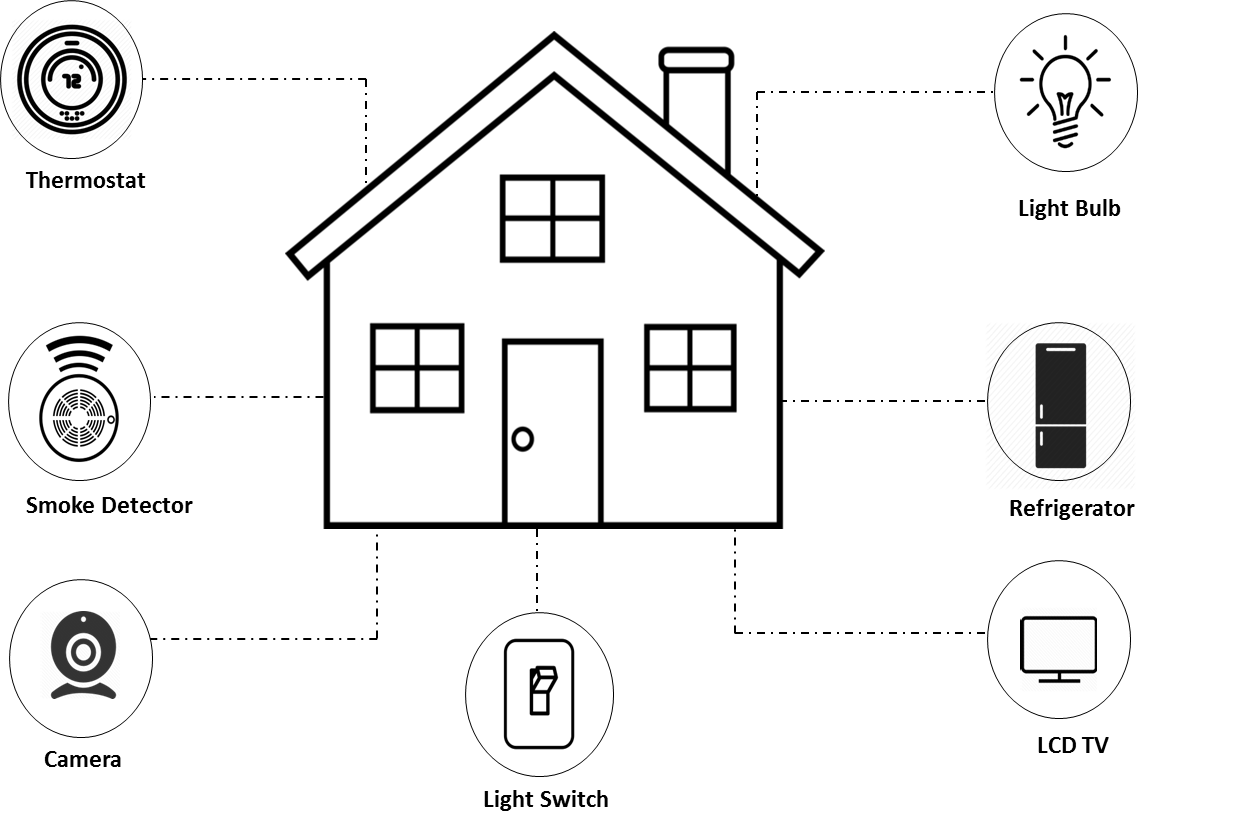
\includegraphics[height=3in]{smart_home_use_case.png}
\end{center}
\caption{Smart home use case Diagram}
\label{smart_home}
\end{figure}


Consider a smart home as illustrated in figure \ref{smart_home} that contains interconnected devices such as a thermostat which automatically detects and regulates the temperature of a room based on prior information of a user's temperature preferences, a smart lock system that can be controlled remotely and informs a user via short messaging when the door has been opened or is closed, a home security camera monitoring system, a smart fridge which sends a reminder when food produce are low. In an event that a malicious intruder attempts  to gain access to the smart lock system and security camera remotely, provenance information can be used to track the series  of events to determine where and how a malicious attack originated. It can also be used as a safeguard to alert of a possible remote or insider compromise thereby protecting against future or current malicious attacks. 





\section{Research Questions}
\textcolor{red}{The unification of data provenance and IoT is essential to the security of data disseminated in an IoT system.} Data provenance and IoT are two essential components that need to be unified. However, the unification of data provenance and IoT raises some important research issues some of which are as a result of pre-existing provenance and IoT related issues. Some of the issues raised as a result of the unification of data provenance with IoT are outlined below:

\begin{itemize}

\item Memory constraints on IoT Devices: The vast amounts of data generated leads to high storage space utilization. Proper memory management and data pruning techniques should be employed for efficient storage of provenance data on memory constrained devices. 

\item A fundamental question exists in effective modeling of provenance data. How do we model provenance data collected from sensors and actuators contained in IoT devices? Are there models used to represent causality between sensor and actuator readings in the IoT architecture.

\item How do we effectively collect provenance data in resource constrained devices and relate this information across various layers of the IoT architecture

\end{itemize}

\section{Research Contribution}

In this dissertation, we propose the following key contributions:

\begin{itemize}
  \item A provenance collection framework which represents causality and dependencies between entities contained in an IoT system. This system creates groundwork for capturing and storing provenance data  across the IoT architectural stack.
  \item A policy driven framework for efficient provenance data storage on IoT devices. We evaluate our contributions for an efficient provenance storage system by using an intrusion detection system on IoT devices.
\end{itemize}

\section{Organization of Dissertation proposal}

The remaining portion of this dissertation proposal is organized as follows. In Chapter 2, we present background information on data provenance and the Internet of Things. We also discuss models for representing provenance data and an overview of relevant compression techniques. In Chapter 3, we outline the literature review on the state of the art on provenance collection in file systems, scientific workflow and database systems. In Chapter 4, we discuss our proposed provenance collection system. We also describe our model construct for representing provenance data cross the IoT architecture. In Chapter 5, we describe our framework for efficient storage of provenance data. Finally, in Chapter 6, we conclude the proposal with proposed future work.

